\chapter{Observation and data reduction}\label{chap:data}
\thispagestyle{fancy}

\section{VLT/MUSE}

NGC 6397 was observed with the Multi Unit Spectroscopic Explorer (MUSE) at the Very Large Telescope (VLT) of the European Southern Observatory (ESO) at Paranal, Chile. MUSE is an integral field spectrograph (IFS). MUSE works by separating the full field of view ($1' \times 1'$) into 24 sub-fields ($2.5" \times 60"$). Each of these 24 is them process by 24 identical but independent integral field units (IFU). Each IFU consists of an image slicer, an spectrograph and a CCD. Each IFU illuminates a $4 \text k \times 4 \text k$ CCD after slicing the light into 48 slit-like slices (with size $\sim 15" \times 0".2$), and decomposing it via a volume phase holographic grating \citep{barden_volume-phase_1998}. The grating achieves a spectral resolution of 1750 at 4650 Å to 3750 at 9300 Å. The data from the 1152 slices is then reconstructed into a $1' \times 1'$ datacube (two spatial and one wavelength axis) with a $0".2$ spatial resolution covering from 4750 Å to 9350 Å sampled at 1.25 Å \citep{bacon_muse_2010}. 

NGC 6397 was observed during the third commissioning period  (ESO Programme ID 60.A-9100(C) \cite{bacon_muse_2014}). The observation were taking from July 26nd to August 3rd, 2014. The observations covered the central part of NGC 6397 ($\sim 3'.5$ from the cluster center see fig~\ref{fig:clustermuse}). The dataset consists of 23 different pointings of MUSE with short exposure times ranging from 25-60 seconds. In total they obtained 127 exposures of the 23 different $1' \times 1'$ regions (see fig~\ref{fig:clustermuse}). This gives a total integration time of 95 minutes for all the observed part of the cluster.


\begin{figure}[H]
        \centering
        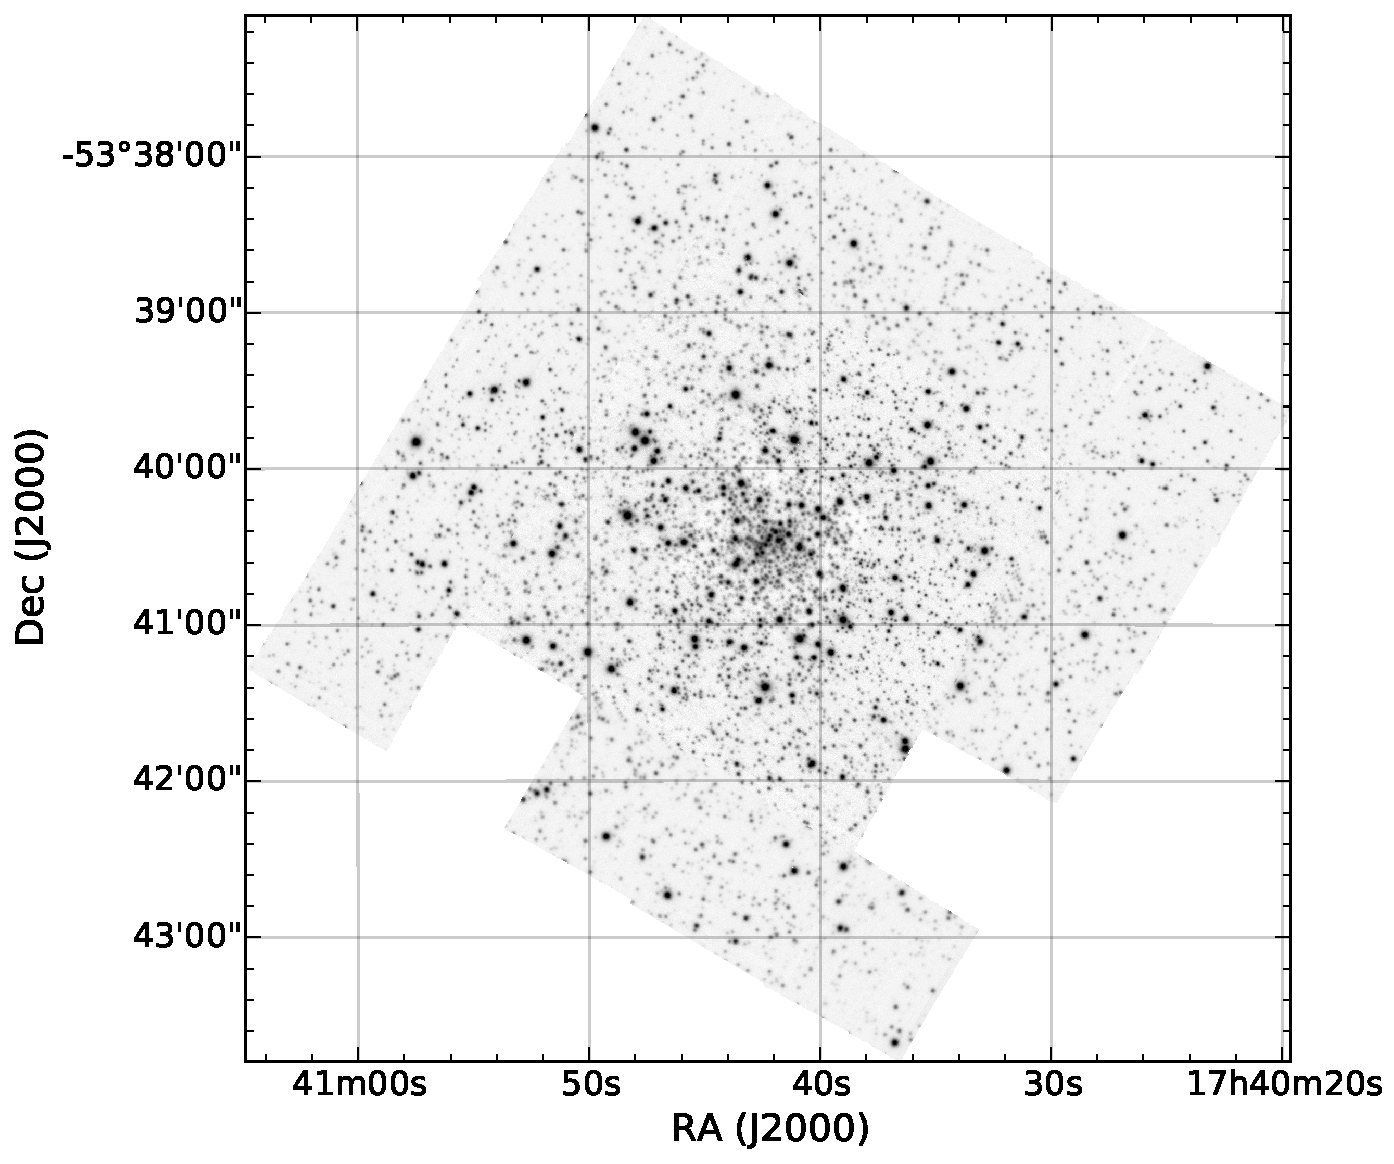
\includegraphics[scale=.6]{assets/images/mosaic.pdf}
\caption{bfagagaga}
\label{fig:clustermuse}
\end{figure}

\section{Processed and Raw data} 

The primary goal of the MUSE observation of NGC 6397 was to create the first comprehensive Hertzsprung-Russell diagram with a sample of over 12 000 spectra \citep{husser_muse_2016}. The large number of spectra obtained allow them to study the kinematics of the globular cluster with the goal to probe the presence of a central black hole in the cluster \citep{kamann_muse_2016}. This data is publicly available thought the \emph{MUSE Science Web Service}\footnote{\url{http://muse-vlt.eu/science/}}. The website contains advanced science products such as reduced datacubes, source catalogs and software tools. For NGC 6397 it can be found the release of the spectra of the globular cluster NGC 6397 as published in the studies mentioned above (\cite{husser_muse_2016} and \cite{kamann_muse_2016}). They provide all the obtained spectra with a signal-to-noise ratio of five or larger, i.e. 14271 spectra in total. For our goal to study the CVs in the globular clusters the data wasn't enough as it mainly covers the range from main sequence to the tip of the red giant branch\footnote{The red giant branch is }. Our approach in this project was to work with the raw science data. The science data can be obtained from the ESO  Science Archive Facility. As stated in the ESO Data Access Policy\footnote{\url{http://archive.eso.org/cms/eso-data-access-policy.html}} all science data is made publicly available through the science archive after the proprietary period (normally one year after the data have been made available to the principal investigator) and all calibration data are public immediately after the observations.  

\subsection{Data Reduction}

The data was reduced with version 1.2.1 of the MUSE Instrument Pipeline Recipes\footnote{The MUSE pipeline can be found at \url{http://www.eso.org/sci/software/pipelines/muse/}}\citep{weilbacher_design_2012}. The pipeline distribution kit includes several packages. The ones used for this work are the following:

\begin{itemize}
        \item The Common Pipeline Library version 6.6 \citep{mckay_common_2004}
        \item The ESO Recipe Execution Tool (EsoRex)\footnote{EsoRex is written by the CPL group (Pipeline System Department) European Southern Observatory \url{http://www.eso.org/sci/software/cpl/esorex.html}} version 3.12.
\end{itemize}

All the data reduction was done calling EsoRex to execute the MUSE DRS recipes from a bash (version 4.3.11) script\footnote{All the configuration files for each of the called MUSE recipes used, the bash scripts, useful python (Python 2.7.6) scripts and other text files relevant for the data reduction can be found at \url{https://github.com/manuelmarcano22/muse2016}} (alternative this can be done via the Python bindings \citep{streicher_python_2012}). We summarize the main steps to produce the fully reduced datacube from the raw science and calibration data download from the ESO Science Archive MUSE Query Form. The data reduction steps can be divided into two categories, pre-processing and post-processing. The pre-processing part includes all the necesarry claibration to remove the instrument signature on the exposures. The post-preocessing then takes the resulting pixel table for each science observation and can resample them to create the datacube.



\begin{enumerate}
        \item Calibration and pre-processing
                \begin{enumerate}[I]
			\item \textbf{Bias substraction}: Bias subtraction was done by combining 10 different bias images into one master bias file. Each bias is part of the calibration files taken by ESO every night. A bias frame is dark image with no exposure time taken to account for the read out noise. (Recipe called \emph{muse\_bias}). For this an all subsequent steps we used a table of additional bad pixels of the CCDs created for the MUSE commission runs. This bad pixel table is distributed along with the MUSE pipeline files. 
			\item \textbf{Flat-fielding}: For the flat-field correction also 10 individual flat frames were combined into a master flat frame. The flat-field images are taking daily at the VLT as part of the standard calibration plan.  The master flat  contains  the  combined  pixel  values  of  the  raw  flat exposures. The purpose is to correct for uneven detector sensitivity. The recipe used was \emph{muse\_flat}. Besides the master flat, the recipe also produces a \emph{trace table} containing polynomials defining the location of the slices on the CCD. 
			\item \textbf{Wavelenght calibration}: For the wavelenght calibration 15 different arc lamp exposures were used. These is 3 per lamp (Ne, Xe, HgCd lamps). The recipe used is \emph{muse\_wavecal}. It detects arc emission lines and determine the wavelength solution for each slice. The goal is to establish the pixel to wavelength equivalence with high precision.
			\item \textbf{Line Spread Function}: The line-spread function is calculated with the recipe \emph{muse\_lsf}. The lines spread function describes the broadening of spectral lines on a CCD. The recipe calculates this  wavelenght dependent function from 15 arc lamp exposures, and the wavelength solution calculated in the step above.  
			\item \textbf{Geometrical calibration}: In this step the recipe \emph{muse\_geometry} can be used to determine where the field of view . This creates a geometry table. A geometry table comes with the standard MUSE pipeline package as a static calibration files. The geometry table prepared for the third commisioning period was used in reducing the data. 
			\item \textbf{Illumination Correction}: Flat-field with sky or twilight flats are taken weekly at the VLT. These are use to do large scale illumination correction. This is done calling the recipe \emph{muse\_twilight}. For the illumination correction also an special purpose  illumination flat field called ILLUM can be used as an input to the recipe. This are taken throught the observing night. We use the one taken closest in time to the science data.  
    \end{enumerate}
\item Post-processing
                \begin{enumerate}[I]
			\item \textbf{Flux calibration}:  In this step a flux response curve from a standard star exposure is created. The end produc of the \emph{muse\_standard} are tables with the response curve as derived from standard star and also the telluric absorption as derived from standard star.
                        \item \textbf{Sky substraction}: Was not done as it is only needed if the observed object fills the fiel of viw that reasonbale sky spectrum cannto be obtained on the obsergationitserf. The sky ubstractionos done dir. No sky  
                        \item \textbf{Astrometry}: Can compute astrometry solution, but the one shppied with the pipeline for the commisiing period was used. 
			\item \textbf{Combination} a full data cube is created from a single exposure, the sky background is removed and the flux calibration and the astrometric calibration, created in the preceding processing steps, are applied. In this step the cubes a sampled to a common value $(0".2 \times 0".2 \times 1.25 \mathring{A})$ . The different for each region of the cluster where merged into a singe datacube and for the center dataxubes of indivial exposures were also created.  
				
				K-means from Creation fo the datacube from the above tables created telluric tables, responese curve, sky cntinuum. Datacibe from single expisures of combining after correctly aligning them creatinan tabkle of ofset. 
                \end{enumerate}
\end{enumerate}


\subsection{Spectra extration and analysis}

The spectra substraction and analysis was carreid wtih QFits View and IRAF \citep{1986SPIE..627..733T}
Astropy \citep{astropy_collaboration_astropy_2013}

Plit

This research made use of APLpy, an open-source plotting package for Python hosted at http://aplpy.github.com

\begin{comment}
s images to form a master
bias, combine 5 lamp-flat exposures, and use one exposure
of each arc lamp to derive the wavelength solution. 11 skyflats,
taken during the evening twilight preceding the science exposures,
were combined and used to create a 3D correction of the
illumination in the range λ = 5000 . . . 8000 Å2
.
The geometry of the instrument was derived f

. These calibrations were found
to be valid for the full period of the first commissioning run of
the instrument and were also shipped with the MUSE pipeline.
i
Pix talbe
he di
erence between sky and
calibration unit illumination. The result of this process is a
large table (hereafter called a pixel-table) for each science frame. This table contains all pixel values corrected for bias and flat-field and their location on the detector. A geometri- cal calibration and the wavelength calibration solution were used to transform the detector coordinate positions to wave- lengths in Ångström and focal plane spatial coordinates 

\end{comment}
